\def\handout{0}   % set to 1 to produce 4-up handouts instead of slides
\def\notes{0}     % set to 1 to show \note{}s
\ifnum\handout=1  % see above for an alternative which uses two preamble files
\documentclass[handout,13pt,compress,c]{beamer}
\usepackage{pgfpages}
\pgfpagesuselayout{4 on 1}[letterpaper,landscape,border shrink=4mm]
\setbeamertemplate{footline}[page number]   % omit if don't want slide number at bottom right
\else
\documentclass[13pt,compress,c]{beamer}
\fi
\usetheme{PaloAlto}
\usepackage{graphicx}
\usepackage{natbib}          % for author year citations \citet \citep
\usepackage{relsize}         % for \smaller etc.
\usepackage{xcolor}
\usepackage{listings}

\graphicspath{ {images/} }

\definecolor{kugreen}{RGB}{50,93,61}
\definecolor{kugreenlys}{RGB}{132,158,139}
\definecolor{kugreenlyslys}{RGB}{173,190,177}
\definecolor{kugreenlyslyslys}{RGB}{214,223,216}

\usecolortheme[named=kugreen]{structure}

\lstset{language=bash,
        basicstyle=\tiny,
        frame=single,
        backgroundcolor=\color{lightgray},
        commentstyle=\color{black},
        showstringspaces=false
        }

\DeclareGraphicsExtensions{.pdf, .jpg, .png}
\setbeamercolor{normal text}{bg=blue!5}
\setbeamertemplate{footline}[page number] % omit if don't want slide number at bottom right
\ifnum\notes=1 \setbeameroption{show notes} \fi
\newcommand{\ft}[1]{\frametitle{#1}}
\newcommand{\bi}{\begin{itemize}}
\newcommand{\ei}{\end{itemize}}
\newcommand{\figw}[2]{\centerline{\includegraphics[width=#2\textwidth]{#1}}}
\newcommand{\figh}[2]{\centerline{\includegraphics[height=#2\textheight]{#1}}}
\newcommand{\fig}[1]{\centerline{\includegraphics{#1}}}
\newcommand{\foot}[1]{\footnotetext{#1}} % smaller text in bottom margin, e.g. citations
\expandafter\def\expandafter\quote\expandafter{\quote\Large}
\makeatletter
\renewcommand\@makefntext[1]{\noindent#1} % see p. 114 of LaTeX Companion 2nd edition
\makeatother
\renewcommand\footnoterule{}
\def\newblock{\hskip .11em plus .33em minus .07em}

\title[GSL code generation]{A brief introduction to GSL code generator}
\author[M. Ryndzionek]{Ryndzionek Mariusz}
\institute{MpicoSys\\ Embedded Pico Systems}
\date{September 2014}
%~~~~~~~~~~~~~~~~~~~~~~~~~~~~~~~~~~~~~~~~~~~~~~~~~~~~~~~~~~~~~~~~~~~~~~~~~~
%~~~~~~~~~~~~~~~~~~~~~~~~~~~~~~~~~~~~~~~~~~~~~~~~~~~~~~~~~~~~~~~~~~~~~~~~~~
%~~~~~~~~~~~~~~~~~~~~~~~~~~~~~~~~~~~~~~~~~~~~~~~~~~~~~~~~~~~~~~~~~~~~~~~~~~
\begin{document}
\frame{\titlepage}
\frame{
   \ft{Outline}
\tableofcontents
}
%~~~~~~~~~~~~~~~~~~~~~~~~~~~~~~~~~~~~~~~~~~~~~~~~~~~~~~~~~~~~~~~~~~~~~~~~~~
%~~~~~~~~~~~~~~~~~~~~~~~~~~~~~~~~~~~~~~~~~~~~~~~~~~~~~~~~~~~~~~~~~~~~~~~~~~
%~~~~~~~~~~~~~~~~~~~~~~~~~~~~~~~~~~~~~~~~~~~~~~~~~~~~~~~~~~~~~~~~~~~~~~~~~~
\section{Motivation}
%~~~~~~~~~~~~~~~~~~~~~~~~~~~~~~~~~~~~~~~~~~~~~~~~~~~~~~~~~~~~~~~~~~~~~~~~~~
%~~~~~~~~~~~~~~~~~~~~~~~~~~~~~~~~~~~~~~~~~~~~~~~~~~~~~~~~~~~~~~~~~~~~~~~~~~
%~~~~~~~~~~~~~~~~~~~~~~~~~~~~~~~~~~~~~~~~~~~~~~~~~~~~~~~~~~~~~~~~~~~~~~~~~~
\frame{
\ft{Software design}
\begin{quote}
''Software design is about overcoming human limitations, not technical ones''\\
\small{--- \textup{Peter Hintjens}, GSL Readme}
\end{quote}
}
%~~~~~~~~~~~~~~~~~~~~~~~~~~~~~~~~~~~~~~~~~~~~~~~~~~~~~~~~~~~~~~~~~~~~~~~~~~
%~~~~~~~~~~~~~~~~~~~~~~~~~~~~~~~~~~~~~~~~~~~~~~~~~~~~~~~~~~~~~~~~~~~~~~~~~~
%~~~~~~~~~~~~~~~~~~~~~~~~~~~~~~~~~~~~~~~~~~~~~~~~~~~~~~~~~~~~~~~~~~~~~~~~~~
\frame{
\ft{Main aspects of becoming a good programmer}
\bi
\item Never throw out anything that works\\(until it is really worn out)
\item Never solve the same problem\\more than once in parallel
\item Solve the same problem often in serial
\item Write code, write code, write code,\\until it is as natural as speaking \ei }
%~~~~~~~~~~~~~~~~~~~~~~~~~~~~~~~~~~~~~~~~~~~~~~~~~~~~~~~~~~~~~~~~~~~~~~~~~~
%~~~~~~~~~~~~~~~~~~~~~~~~~~~~~~~~~~~~~~~~~~~~~~~~~~~~~~~~~~~~~~~~~~~~~~~~~~
%~~~~~~~~~~~~~~~~~~~~~~~~~~~~~~~~~~~~~~~~~~~~~~~~~~~~~~~~~~~~~~~~~~~~~~~~~~
\section{Introduction}
%~~~~~~~~~~~~~~~~~~~~~~~~~~~~~~~~~~~~~~~~~~~~~~~~~~~~~~~~~~~~~~~~~~~~~~~~~~
%~~~~~~~~~~~~~~~~~~~~~~~~~~~~~~~~~~~~~~~~~~~~~~~~~~~~~~~~~~~~~~~~~~~~~~~~~~
%~~~~~~~~~~~~~~~~~~~~~~~~~~~~~~~~~~~~~~~~~~~~~~~~~~~~~~~~~~~~~~~~~~~~~~~~~~
\frame{
\ft{Tackling Complexity}
\bi \item Making a language general purpose is a mistaken approach \ei
\begin{quote}
''Complexity is difficult to control, and complex languages (like Perl and C++)\\
have a reputation for producing complex and hard-to-maintain code.''\\
\small{--- \textup{Peter Hintjens}, GSL Readme}
\end{quote}
\bi \item Instead create domain specific models and translate them to code \ei
}
%~~~~~~~~~~~~~~~~~~~~~~~~~~~~~~~~~~~~~~~~~~~~~~~~~~~~~~~~~~~~~~~~~~~~~~~~~~
%~~~~~~~~~~~~~~~~~~~~~~~~~~~~~~~~~~~~~~~~~~~~~~~~~~~~~~~~~~~~~~~~~~~~~~~~~~
%~~~~~~~~~~~~~~~~~~~~~~~~~~~~~~~~~~~~~~~~~~~~~~~~~~~~~~~~~~~~~~~~~~~~~~~~~~
\frame{
\ft{Abstract languages - Hammer Principle}
\begin{quote}
''if all you have is a hammer, everything looks like a nail''
\end{quote}
\vfill
\begin{center}
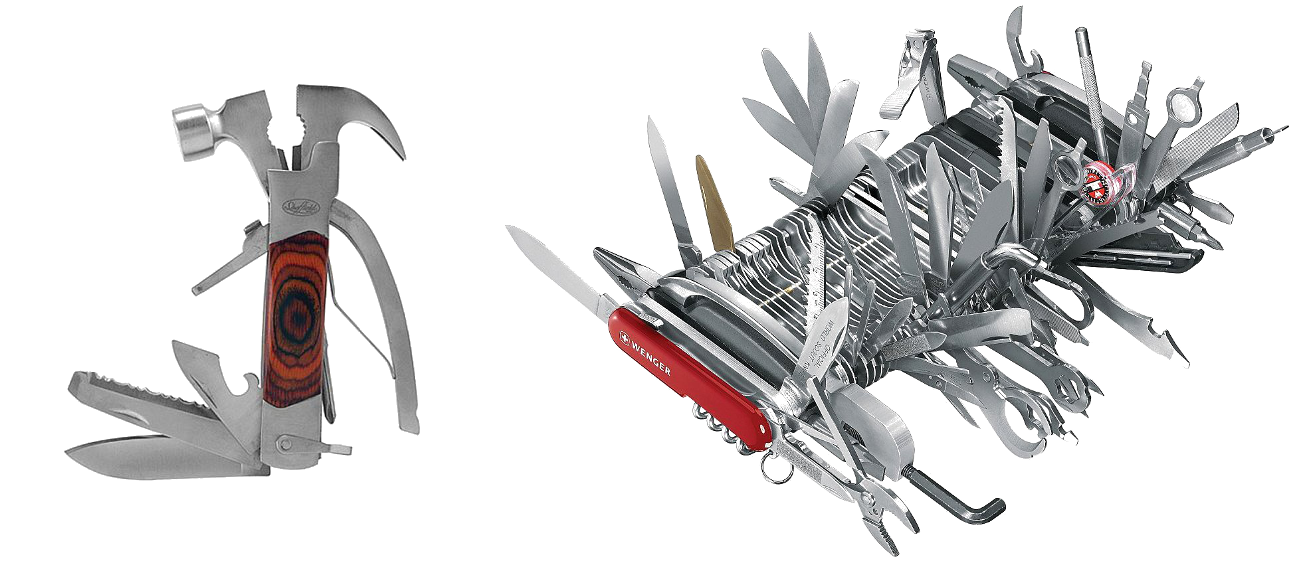
\includegraphics[width=\textwidth]{swiss_hammer.png}
\end{center}
}
%~~~~~~~~~~~~~~~~~~~~~~~~~~~~~~~~~~~~~~~~~~~~~~~~~~~~~~~~~~~~~~~~~~~~~~~~~~
%~~~~~~~~~~~~~~~~~~~~~~~~~~~~~~~~~~~~~~~~~~~~~~~~~~~~~~~~~~~~~~~~~~~~~~~~~~
%~~~~~~~~~~~~~~~~~~~~~~~~~~~~~~~~~~~~~~~~~~~~~~~~~~~~~~~~~~~~~~~~~~~~~~~~~~
\frame{
\ft{Myths}
\bi
\item Code generators only work for simplistic cases
\item Generated code is unreadable, and generated code is low quality
\item Code generators are expensive to make
\item Code generators are too much effort to use
\item Code generators are complex
\ei
}
%~~~~~~~~~~~~~~~~~~~~~~~~~~~~~~~~~~~~~~~~~~~~~~~~~~~~~~~~~~~~~~~~~~~~~~~~~~
%~~~~~~~~~~~~~~~~~~~~~~~~~~~~~~~~~~~~~~~~~~~~~~~~~~~~~~~~~~~~~~~~~~~~~~~~~~
%~~~~~~~~~~~~~~~~~~~~~~~~~~~~~~~~~~~~~~~~~~~~~~~~~~~~~~~~~~~~~~~~~~~~~~~~~~
\frame{
\ft{Pros}
\bi
\item We have to write much less code to get the same results
\item You can create near-perfect abstractions that map to your real world
\item We get high-level models of important aspects of the system
\item We can produce extremely high-quality code
\item We write less internal documentation, and often none at all
\item We are immune to technological changes
\item Non-programmers can maintain a project
\ei
}
%~~~~~~~~~~~~~~~~~~~~~~~~~~~~~~~~~~~~~~~~~~~~~~~~~~~~~~~~~~~~~~~~~~~~~~~~~~
%~~~~~~~~~~~~~~~~~~~~~~~~~~~~~~~~~~~~~~~~~~~~~~~~~~~~~~~~~~~~~~~~~~~~~~~~~~
%~~~~~~~~~~~~~~~~~~~~~~~~~~~~~~~~~~~~~~~~~~~~~~~~~~~~~~~~~~~~~~~~~~~~~~~~~~
\frame{
\ft{Cons}
\bi
\item People do not rapidly understand or trust the approach
\item Programmers do not rapidly understand the models
\item Quickly excludes other people (pro or con ?)
\ei
}
%~~~~~~~~~~~~~~~~~~~~~~~~~~~~~~~~~~~~~~~~~~~~~~~~~~~~~~~~~~~~~~~~~~~~~~~~~~
%~~~~~~~~~~~~~~~~~~~~~~~~~~~~~~~~~~~~~~~~~~~~~~~~~~~~~~~~~~~~~~~~~~~~~~~~~~
%~~~~~~~~~~~~~~~~~~~~~~~~~~~~~~~~~~~~~~~~~~~~~~~~~~~~~~~~~~~~~~~~~~~~~~~~~~
\frame{
\ft{How does it work ?}
\vfill
\begin{center}
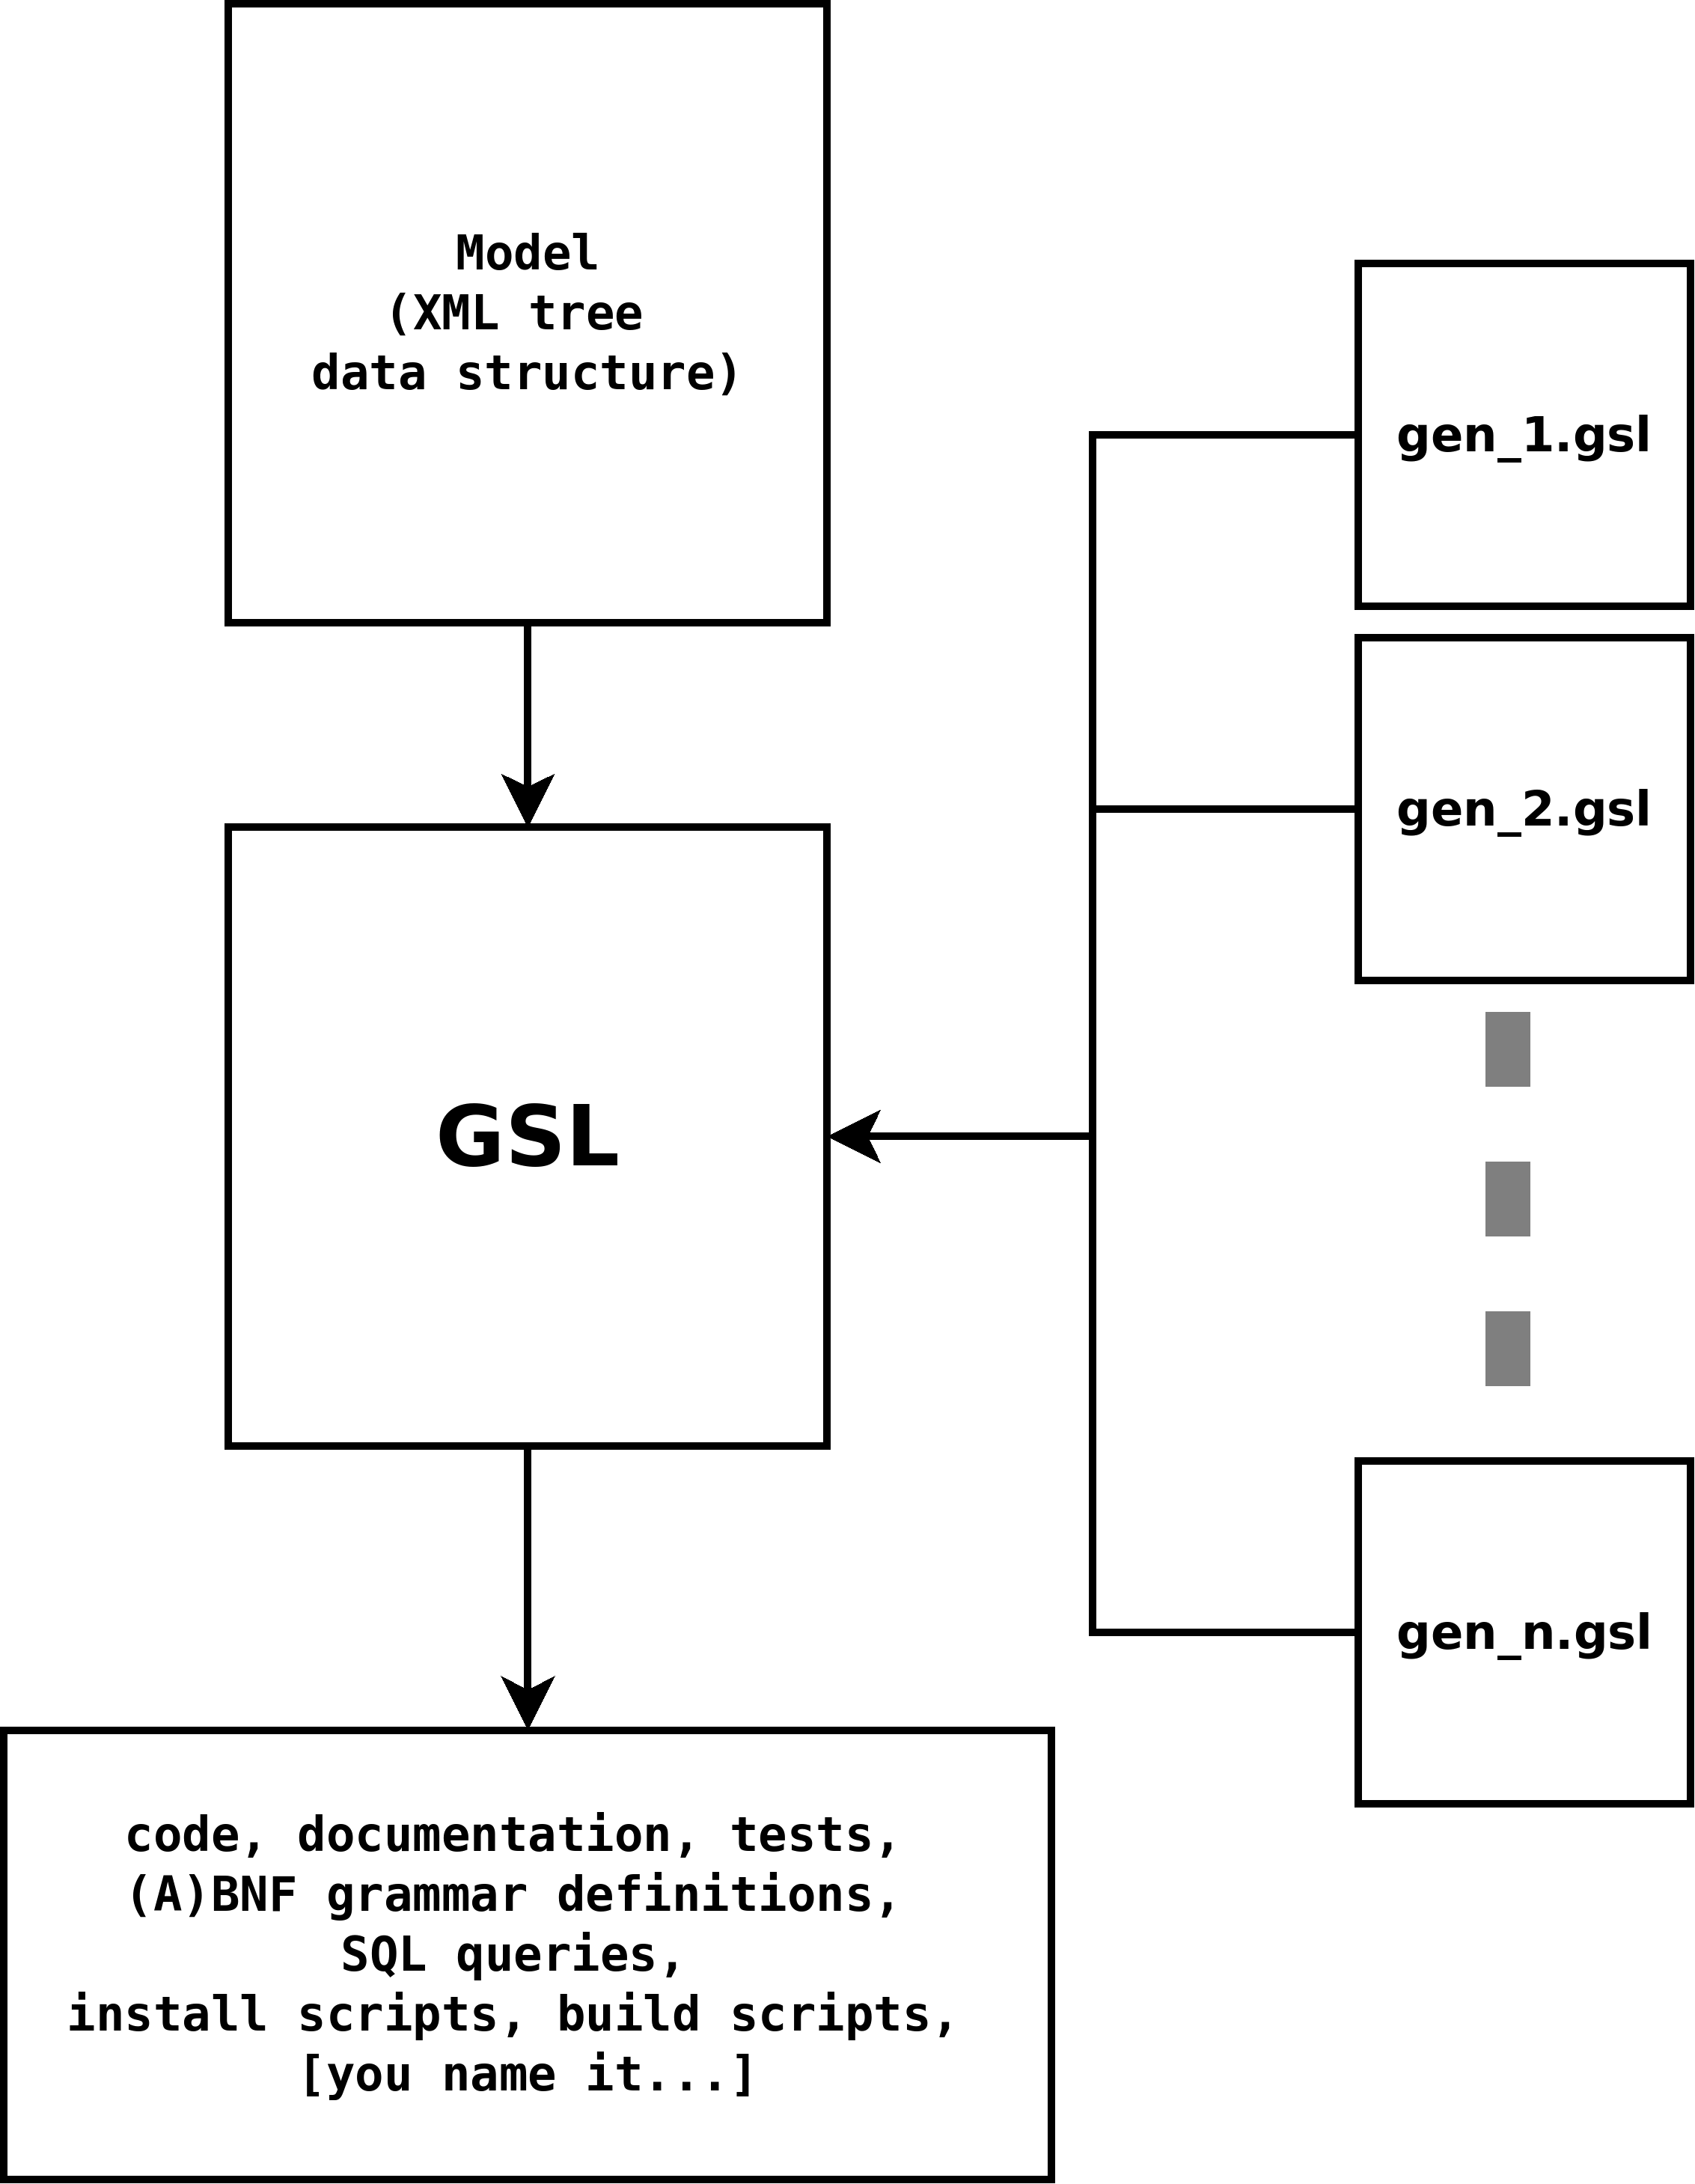
\includegraphics[width=0.4\textwidth]{how.png}
\end{center}
}
%~~~~~~~~~~~~~~~~~~~~~~~~~~~~~~~~~~~~~~~~~~~~~~~~~~~~~~~~~~~~~~~~~~~~~~~~~~
%~~~~~~~~~~~~~~~~~~~~~~~~~~~~~~~~~~~~~~~~~~~~~~~~~~~~~~~~~~~~~~~~~~~~~~~~~~
%~~~~~~~~~~~~~~~~~~~~~~~~~~~~~~~~~~~~~~~~~~~~~~~~~~~~~~~~~~~~~~~~~~~~~~~~~~
\section{Some details}
%~~~~~~~~~~~~~~~~~~~~~~~~~~~~~~~~~~~~~~~~~~~~~~~~~~~~~~~~~~~~~~~~~~~~~~~~~~
%~~~~~~~~~~~~~~~~~~~~~~~~~~~~~~~~~~~~~~~~~~~~~~~~~~~~~~~~~~~~~~~~~~~~~~~~~~
%~~~~~~~~~~~~~~~~~~~~~~~~~~~~~~~~~~~~~~~~~~~~~~~~~~~~~~~~~~~~~~~~~~~~~~~~~~
\frame{
\ft{How does it look like ?}
\vfill
\begin{center}
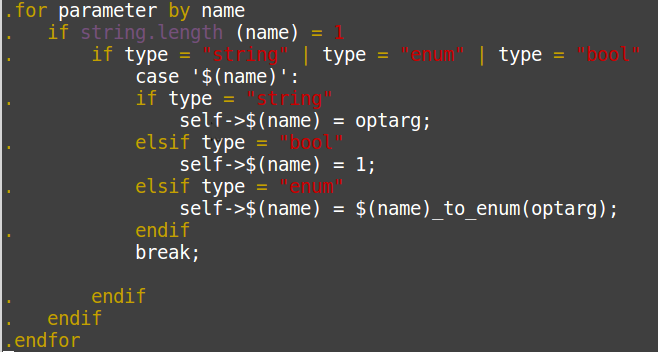
\includegraphics[width=0.8\textwidth]{look.png}
\end{center}
}
%~~~~~~~~~~~~~~~~~~~~~~~~~~~~~~~~~~~~~~~~~~~~~~~~~~~~~~~~~~~~~~~~~~~~~~~~~~
%~~~~~~~~~~~~~~~~~~~~~~~~~~~~~~~~~~~~~~~~~~~~~~~~~~~~~~~~~~~~~~~~~~~~~~~~~~
%~~~~~~~~~~~~~~~~~~~~~~~~~~~~~~~~~~~~~~~~~~~~~~~~~~~~~~~~~~~~~~~~~~~~~~~~~~
\frame{
\ft{How does it look like ?}
\vfill
\begin{center}
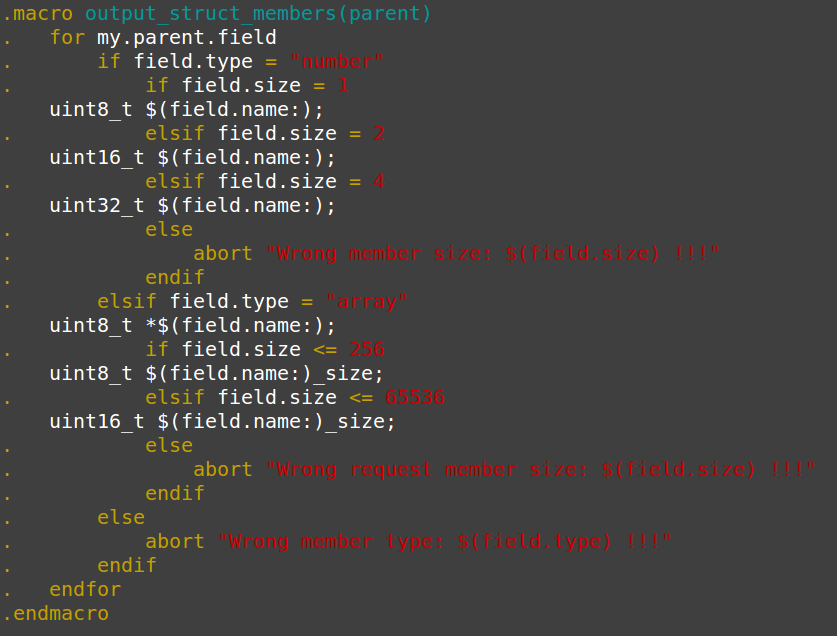
\includegraphics[width=0.8\textwidth]{look_2.png}
\end{center}
}
%~~~~~~~~~~~~~~~~~~~~~~~~~~~~~~~~~~~~~~~~~~~~~~~~~~~~~~~~~~~~~~~~~~~~~~~~~~
%~~~~~~~~~~~~~~~~~~~~~~~~~~~~~~~~~~~~~~~~~~~~~~~~~~~~~~~~~~~~~~~~~~~~~~~~~~
%~~~~~~~~~~~~~~~~~~~~~~~~~~~~~~~~~~~~~~~~~~~~~~~~~~~~~~~~~~~~~~~~~~~~~~~~~~
\frame{
\ft{How does it look like ?}
XML transformations - creating, defining and deleting XML elements
\vfill
\begin{center}
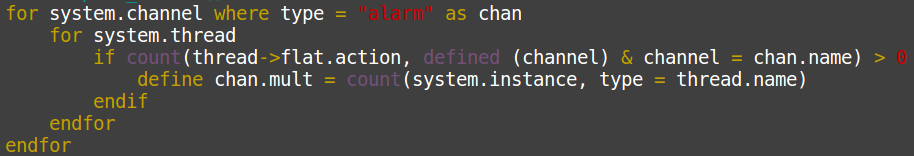
\includegraphics[width=1.0\textwidth]{xml_manip.png}
\end{center}
}
%~~~~~~~~~~~~~~~~~~~~~~~~~~~~~~~~~~~~~~~~~~~~~~~~~~~~~~~~~~~~~~~~~~~~~~~~~~
%~~~~~~~~~~~~~~~~~~~~~~~~~~~~~~~~~~~~~~~~~~~~~~~~~~~~~~~~~~~~~~~~~~~~~~~~~~
%~~~~~~~~~~~~~~~~~~~~~~~~~~~~~~~~~~~~~~~~~~~~~~~~~~~~~~~~~~~~~~~~~~~~~~~~~~
\begin{frame}[fragile]
\frametitle{Some interesting properties}
Substitution pretty-print modifiers -- avoiding ''visual smog''

\begin{semiverbatim}
\begin{lstlisting}
        $( <expression> [% format] [: pretty-print] )
        Examples:
            var = "Code generation using GSL"
            $(var) -> "code generation using gsl"
            $(Var) -> "Code Generation Using GSL"
            $(var:) or $(var:no) - > "Code generation using GSL"
            $(var:c) -> "code_generation_using_gsl"
            $(VAR) -> "CODE GENERATION USING GSL"

/*  $("Description:":block)\
                  $(var:justify,block%-8s)  */

/*  Description:  code                              */
/*                geneartion                        */
/*                using                             */
/*                gsl                               */

\end{lstlisting}
\end{semiverbatim}
\end{frame}
%~~~~~~~~~~~~~~~~~~~~~~~~~~~~~~~~~~~~~~~~~~~~~~~~~~~~~~~~~~~~~~~~~~~~~~~~~~
%~~~~~~~~~~~~~~~~~~~~~~~~~~~~~~~~~~~~~~~~~~~~~~~~~~~~~~~~~~~~~~~~~~~~~~~~~~
%~~~~~~~~~~~~~~~~~~~~~~~~~~~~~~~~~~~~~~~~~~~~~~~~~~~~~~~~~~~~~~~~~~~~~~~~~~
\frame{
\ft{Some interesting properties}
\bi
\item Fully recurrent macros and functions
\item Shuffling
\item Configurable line terminators and escape symbols
\item Large number of built-in functions
\ei
}
%~~~~~~~~~~~~~~~~~~~~~~~~~~~~~~~~~~~~~~~~~~~~~~~~~~~~~~~~~~~~~~~~~~~~~~~~~~
%~~~~~~~~~~~~~~~~~~~~~~~~~~~~~~~~~~~~~~~~~~~~~~~~~~~~~~~~~~~~~~~~~~~~~~~~~~
%~~~~~~~~~~~~~~~~~~~~~~~~~~~~~~~~~~~~~~~~~~~~~~~~~~~~~~~~~~~~~~~~~~~~~~~~~~
\frame{
\ft{Real-life example}
getopt commandline parser generator
\vfill
\begin{center}
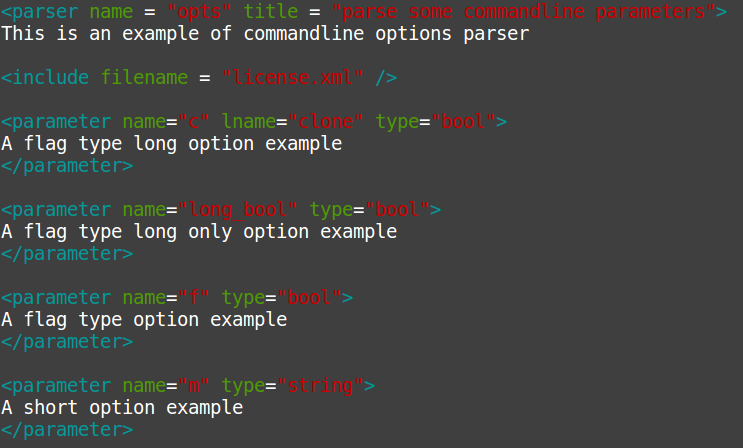
\includegraphics[width=1.0\textwidth]{parser.png}
\end{center}
}
%~~~~~~~~~~~~~~~~~~~~~~~~~~~~~~~~~~~~~~~~~~~~~~~~~~~~~~~~~~~~~~~~~~~~~~~~~~
%~~~~~~~~~~~~~~~~~~~~~~~~~~~~~~~~~~~~~~~~~~~~~~~~~~~~~~~~~~~~~~~~~~~~~~~~~~
%~~~~~~~~~~~~~~~~~~~~~~~~~~~~~~~~~~~~~~~~~~~~~~~~~~~~~~~~~~~~~~~~~~~~~~~~~~
\frame{
\ft{Real-life example}
getopt commandline parser generator
\vfill
\begin{center}
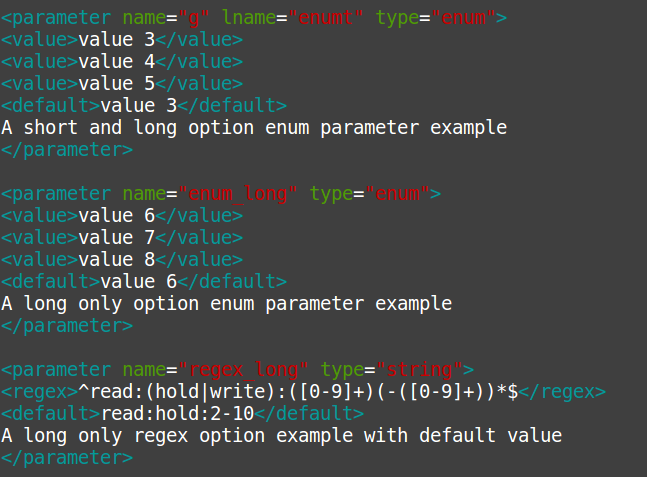
\includegraphics[width=0.8\textwidth]{parser_2.png}
\end{center}
}
%~~~~~~~~~~~~~~~~~~~~~~~~~~~~~~~~~~~~~~~~~~~~~~~~~~~~~~~~~~~~~~~~~~~~~~~~~~
%~~~~~~~~~~~~~~~~~~~~~~~~~~~~~~~~~~~~~~~~~~~~~~~~~~~~~~~~~~~~~~~~~~~~~~~~~~
%~~~~~~~~~~~~~~~~~~~~~~~~~~~~~~~~~~~~~~~~~~~~~~~~~~~~~~~~~~~~~~~~~~~~~~~~~~
\frame{
\ft{Real-life example}
Diff after adding new option
\vfill
\begin{center}
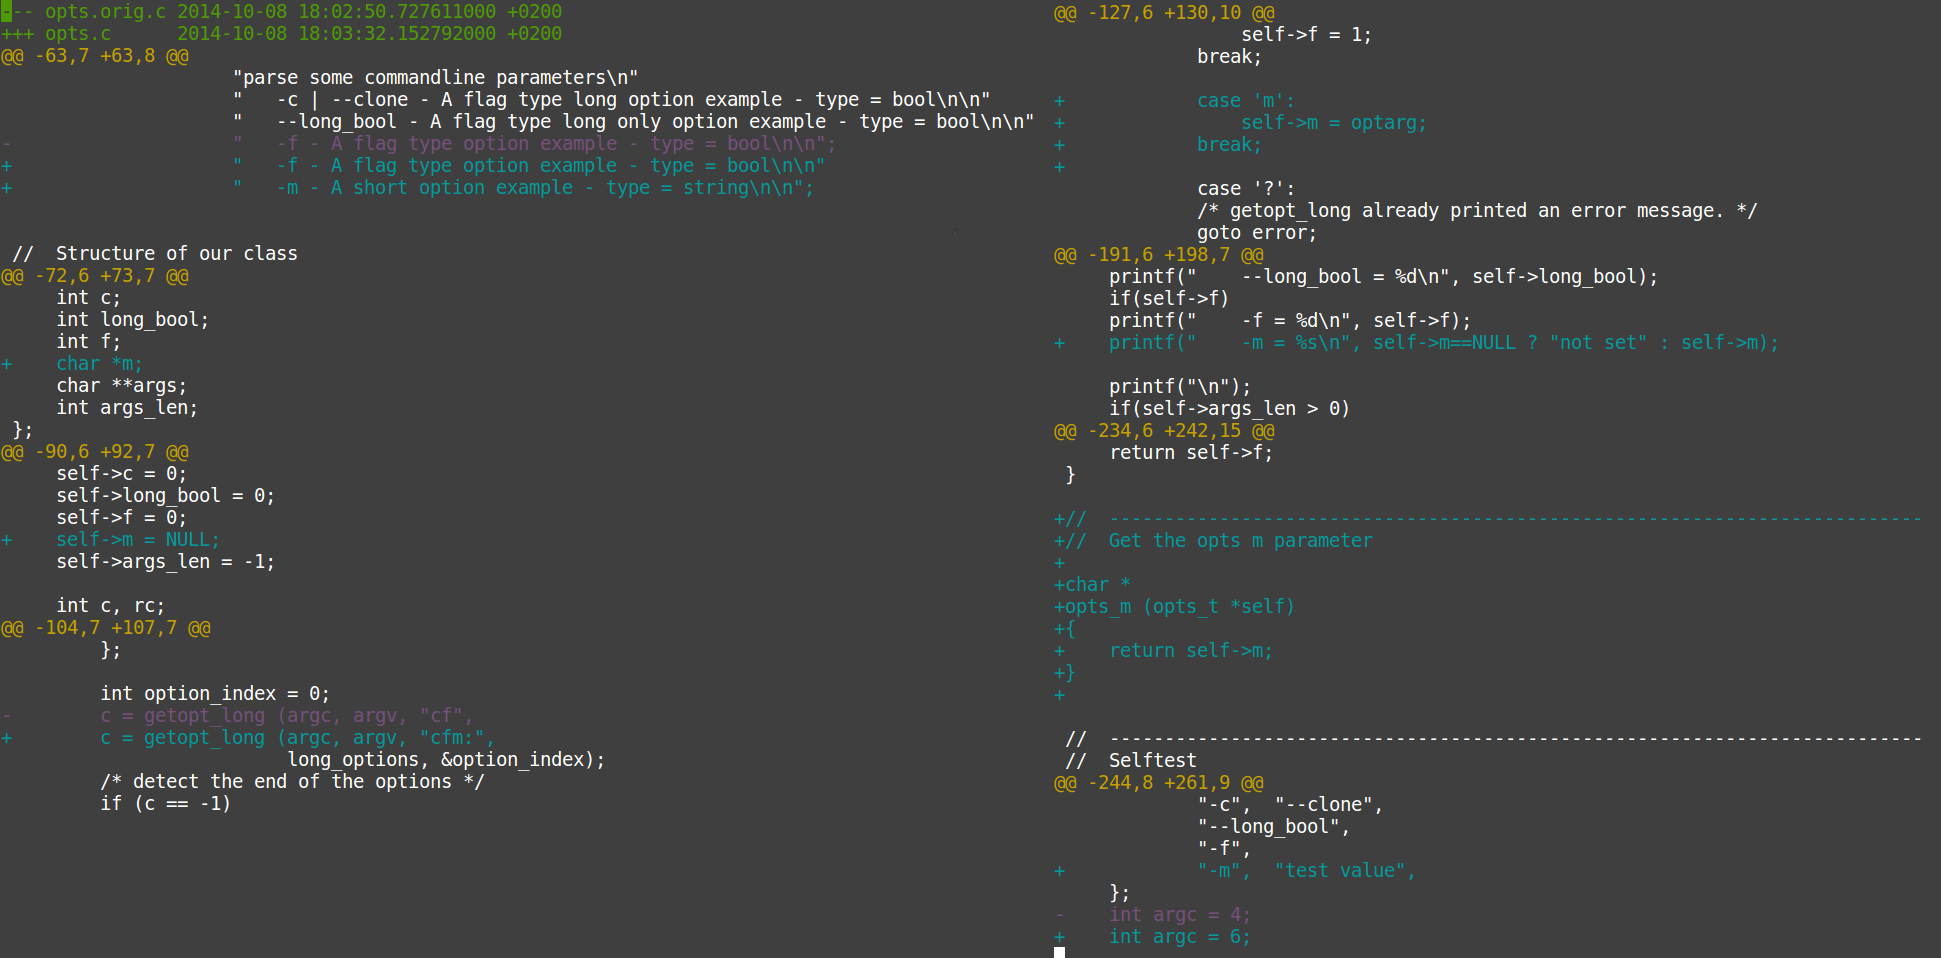
\includegraphics[width=1.0\textwidth]{diff.png}
\end{center}
}
%~~~~~~~~~~~~~~~~~~~~~~~~~~~~~~~~~~~~~~~~~~~~~~~~~~~~~~~~~~~~~~~~~~~~~~~~~~
%~~~~~~~~~~~~~~~~~~~~~~~~~~~~~~~~~~~~~~~~~~~~~~~~~~~~~~~~~~~~~~~~~~~~~~~~~~
%~~~~~~~~~~~~~~~~~~~~~~~~~~~~~~~~~~~~~~~~~~~~~~~~~~~~~~~~~~~~~~~~~~~~~~~~~~
\frame{
\begin{center}
\textbf{THE END}
\end{center}
}
\end{document}
